\frontmatter												%Seitennumerierung
\pagenumbering{Roman}										%Römische Zahlen
\addtocounter{page}{2}

\newcommand{\doublesignature}[2]{%
  \parbox{\textwidth}{
    \hfill
    \parbox{7cm}{
      \centering
      \rule{6cm}{1pt}\\
      #1
    }
    \parbox{7cm}{
      \centering
      \rule{6cm}{1pt}\\
      #2
    }
  }
  \mbox{}\\
  \mbox{}\\
  \mbox{}\\
  \mbox{}\\
}
\newcommand{\singlesignature}[2]{%
  \parbox{\textwidth}{
    \hfill
    \parbox{7cm}{
      \centering
      \rule{6cm}{1pt}\\
      #1
    }
  }
  \mbox{}\\
  \mbox{}\\
  \mbox{}\\
  \mbox{}\\
}

\vspace*{20pt}

\section*{Eidesstattliche Erklärung}
\label{sec:eidesstattliche-erklaerung}
Ich erkläre an Eides statt, dass ich die vorliegende Arbeit selbstständig verfasst, andere als die angegebenen
Quellen/Hilfsmittel nicht benutzt und die den benutzten Quellen wörtlich und inhaltlich entnommenen
Stellen als solche kenntlich gemacht habe.\\
\\
Arnfels, am 18. März 2020\\

\vskip 1cm

\doublesignature{Stefan Hörmann}{Nicolas Perl}
\singlesignature{Alois Vollmaier}

\vskip 5cm

\clearpage

\newpage
\thispagestyle{empty}
\mbox{}

\clearpage

\section*{Danksagung}
\label{sec:danksagung}
An dieser Stelle möchten wir, Stefan Hörmann, Nicolas Perl und Alois Vollmaier, uns im Rahmen der Diplomarbeit bei allen bedanken, die uns unterstützt und betreut haben.
Insbesondere sind dies einerseits unsere Betreuer, Dipl.-Ing Dr. Gerhand Pretterhofer und Dipl.-Ing Manfred Steiner.
Mithilfe deren fundamental wichtigen Ideen und deren Fachwissen ist es uns gelungen, dieses Werk zu kreieren.
Außerdem möchten wir uns herzlich bei Herrn Ing. Konrad Wilhelm, Herrn Ing. Dipl.-Päd. St.-Rat Reinhard Semlitsch und Herrn Franz Skof bedanken, welche uns beim Fertigungsprozess enorm unterstützten und eine elementare Rolle spielten.
Nicht zuletzt gebührt ein ganz spezieller Dank unseren Familien, Verwandten und Freunden, welche und in dieser einschneidenten Zeit voll uns ganz unterstützten.
\clearpage

\newpage
\thispagestyle{empty}
\mbox{}

\clearpage

\section*{Abstract}
\label{sec:abstract}
The goal of this diploma thesis is to create a machine which is able to shuffle and dispense playing cards.
The main idea is to create these processes as space and time efficient as possible.
In order to achieve these goals, the entire project is split into the segments mechanics, electronics and programming.
Each of these subdivisions is assigned to a separate team member.
The task of the mechanical part consists of the mentioned machine, adapted to the requirements.
Furthermore, calculations of elementary important and a partial construction shall be implemented.
The electrical part of this diploma thesis includes the design and the development of an electrical circuit and its corresponding printed circuit board as well as its layout and its assembly.
A commissioning and the execution of tests shall also be made.
The task of the informatics subdivision is to program a user-friendly, graphical interface and to establish communication between a Raspberry Pi and a microcontroller.
\section*{Zusammenfassung}
Wir setzten uns als Ziel, eine Maschine zu entwickeln, welche das Mischen sowie das Ausgeben von Spielkarten übernimmt.
Die Idee ist es, dieses Verfahren möglichst platzsparend und zeiteffizient zu realisieren.
Um genannte Ziele zu erfüllen, wird das gesamte Projekt in die Teilbereiche Mechanik, Elektronik und Informatik aufgeteilt, wobei jeder Teilbereich einem Teammitglied zugeordnet werden soll.
Die Arbeit des mechanischen Teils besteht darin, die genannte Maschine, angepasst an die gestellten Anforderungen, zu konstruieren.
Weiters sollen Berechnungen von elementar wichtigen Baugruppen erstellt sowie ein Teilaufbau gemacht werden.
Der elektrische Teil dieser Diplomarbeit umfasst das Entwerfen und das Entwickeln eines Schaltplans
und einer dazugehörigen Leiterplatte sowie das Layouten dieser und deren Bestückung.
Eine Inbetriebnahme und das Durchführen von Tests soll ebenfalls vorgenommen werden.
Die Aufgabe des informatischen Teilbereichs ist es, eine benutzerfreundliche, grafische Oberfläche zu programmieren sowie eine Kommunikation zwischen einem Raspberry Pi und einem Microcontroller herzustellen.
\clearpage

\newpage
\thispagestyle{empty}
\mbox{}

\clearpage

\subsection*{Gender Erklärung}
\label{sec:gender-erklaerung}
Aus Gründen der besseren Lesbarkeit wird in dieser Arbeit die Sprachform des generischen Maskulinums angewendet.
Es wird an dieser Stelle darauf hingewiesen, dass die ausschließliche Verwendung der männlichen Form geschlechtsunabhängig verstanden werden soll.

\subsection*{Über dieses Dokument}
\label{sec:ueber-dokument}
Diese Arbeit wurde in \LaTeX{} verfasst.
Diese Art der Dokumentation bietet gegenüber den normalen Textverarbeitungen gewisse Vorteile hinsichtlich der Formatierung und des Einbindens von Grafiken.
Auch Formeln können sehr einfach und effizient angegegeben werden. Die Rohfassung des Dokuments befindet sich auf dem Arnfelser Gitweb Server der HTBLA Kaindorf Abteilung Mechatronik.

\subsection*{Erklärung der Sprachen}
\label{sec:erklärung-sprachen}
Da viele Ausdrücke, Datenblätter und weitere technische Dokumente in Englisch verwendet werden, lässt sich eine teilweise Vermengung der Sprachen nicht vermeiden.
\clearpage

\newpage
\thispagestyle{empty}
\mbox{}

\clearpage

\section*{Projektteam}
\label{sec:projektteam}

\subsection*{Stefan Hörmann}
\begin{wrapfigure}[10]{0}{0.5\textwidth}
\begin{center}
  \vspace{-20mm}
  
\includegraphics[width=0.3\textwidth]{fig/H.jpg}
\end{center}
\end{wrapfigure}
\mbox{}\\
\mbox{}\\
\textbf{Aufgabenbereich}:\\
Mechanik\\
\textbf{Betreuer}:\\
Dr. Dipl-Ing. Gerhard Pretterhofer
\mbox{}\\
\mbox{}\\
\mbox{}\\
\subsection*{Nicolas Perl}
\begin{wrapfigure}[10]{0}{0.5\textwidth}
\begin{center}
  \vspace{-20mm}
  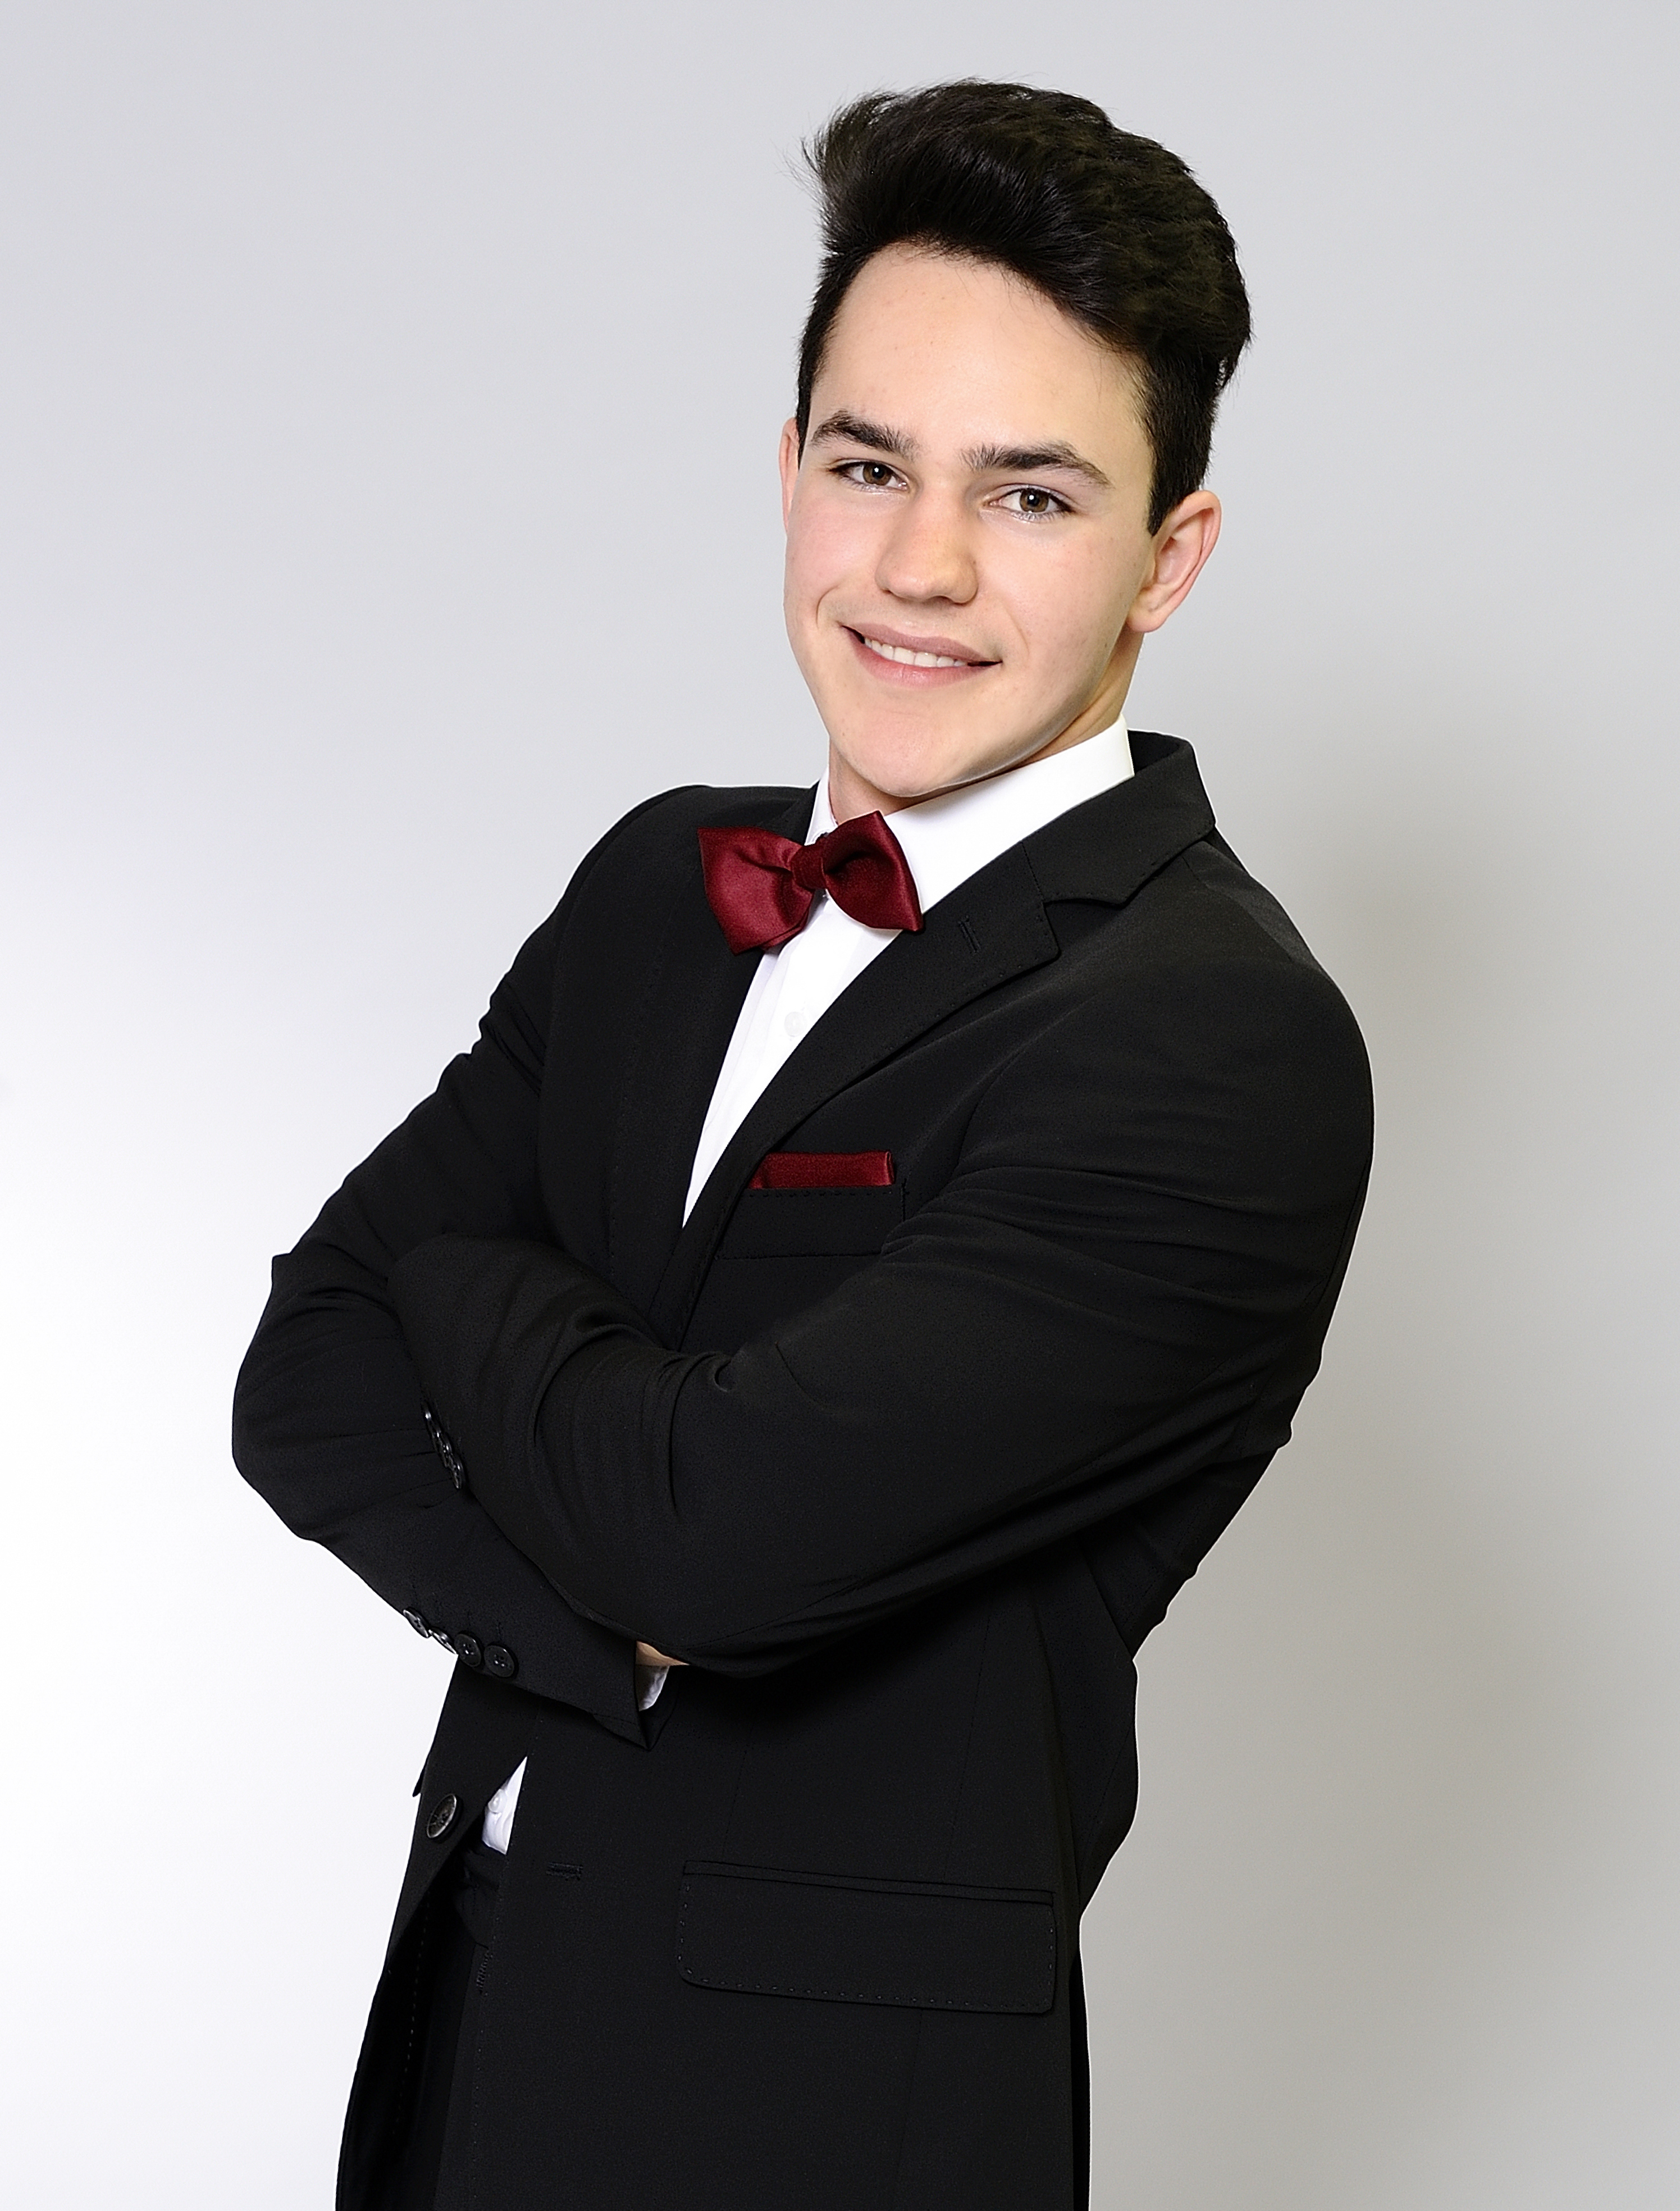
\includegraphics[width=0.3\textwidth]{fig/P.jpg}
\end{center}
\end{wrapfigure}
\mbox{}\\
\mbox{}\\
\textbf{Aufgabenbereich}:\\
Elektronik\\
\textbf{Betreuer}:\\
Dipl-Ing. Manfred Steiner
\mbox{}\\
\mbox{}\\
\mbox{}\\
\subsection*{Alois Vollmaier}
\begin{wrapfigure}[10]{0}{0.5\textwidth}
\begin{center}
  \vspace{-20mm}
  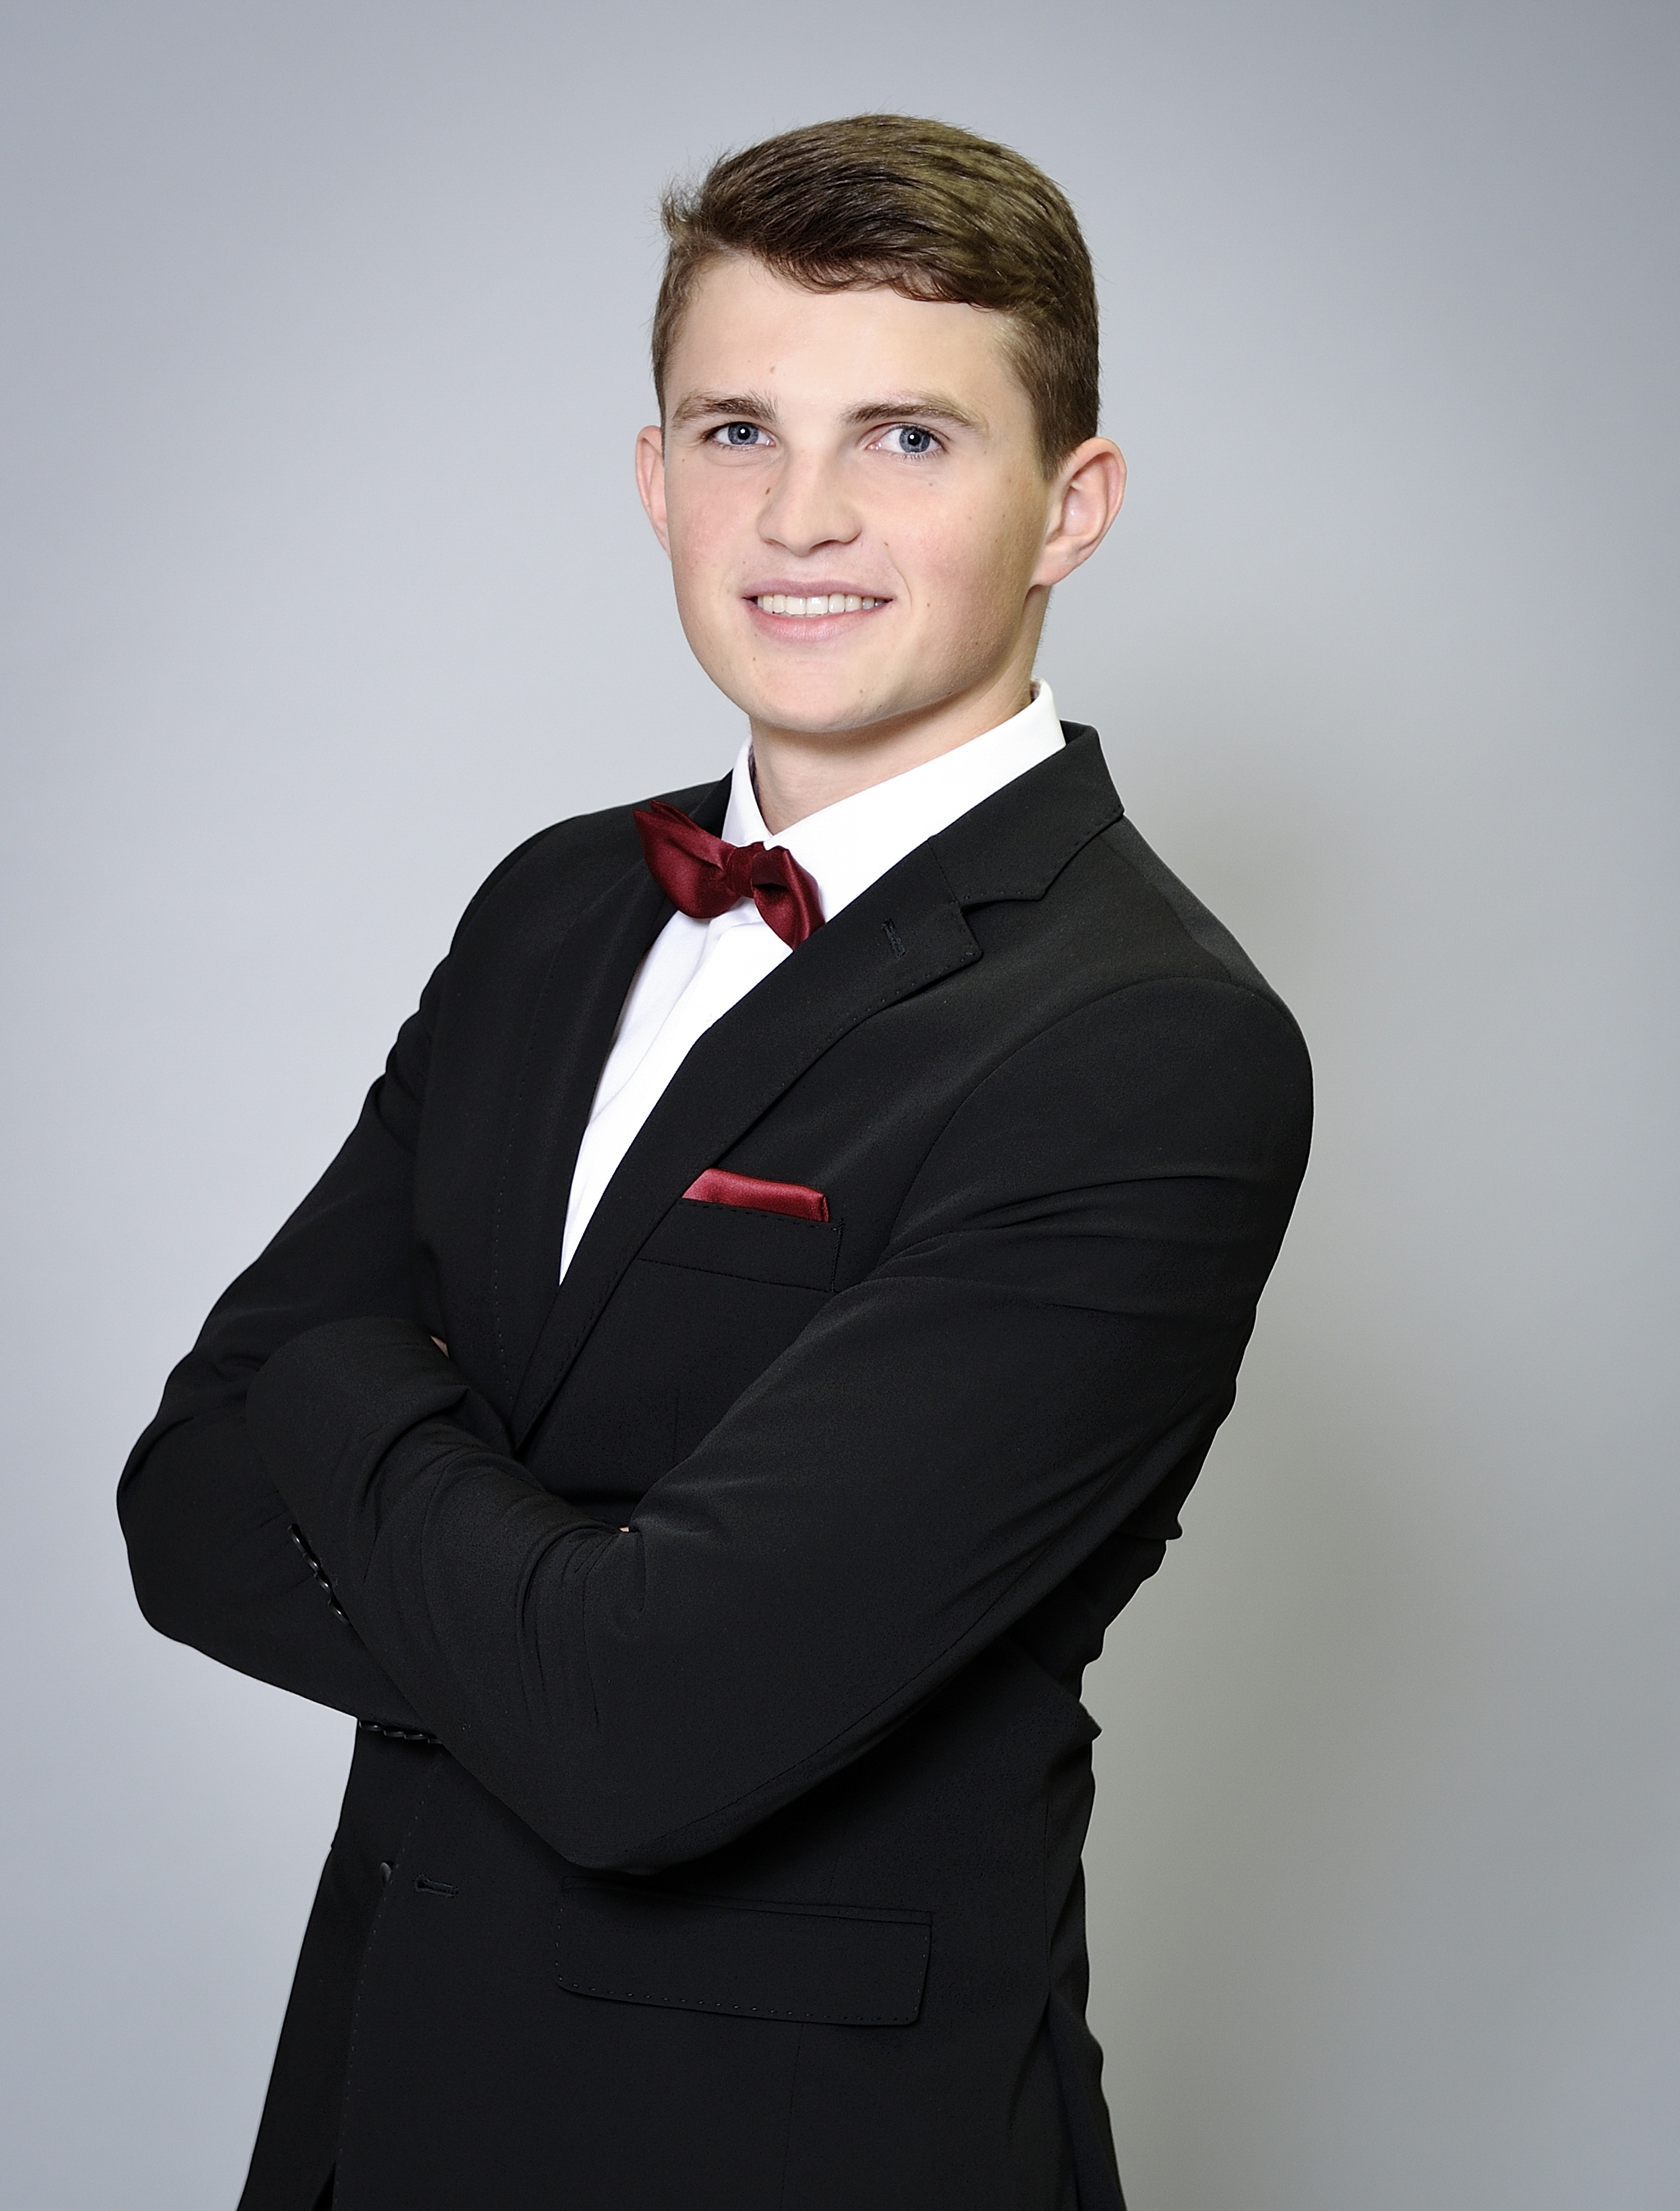
\includegraphics[width=0.3\textwidth]{fig/V.jpg}
\end{center}
\end{wrapfigure}
\mbox{}\\
\mbox{}\\
\textbf{Aufgabenbereich}:\\
Informatik\\
\textbf{Betreuer}:\\
Dipl-Ing. Manfred Steiner
\mbox{}\\
\mbox{}\\
\mbox{}\\
\mbox{}\\
\mbox{}\\
\mbox{}\\